\section{Conclusion et perspectives}
\begin{frame}
\frametitle{Combien d'utilisateurs ?}
\begin{columns}[c]
\column{0.5\textwidth}
\begin{block}{Difficile à dire \ldots}
\begin{itemize}
    \item $\approx$ 600 membres sur la liste utilisateurs
    \item $\approx$ Entre 100 et 150 messages par mois
    \item $\approx$ 100 membres sur la liste développeurs
    \item $\approx$ 118 comptes sur le système de gestion des bugs
    \item $\approx$ 50 contributeurs (listé dans la documentation)
    \item $\approx$ 3400 téléchargements for OTB 5.0
  \end{itemize}
\end{block}
\begin{block}{Users Days 2015, 2016 et 2017}
  40 à 60 participants à Toulouse pendant 3 jours
\end{block}
\column{0.5\textwidth}
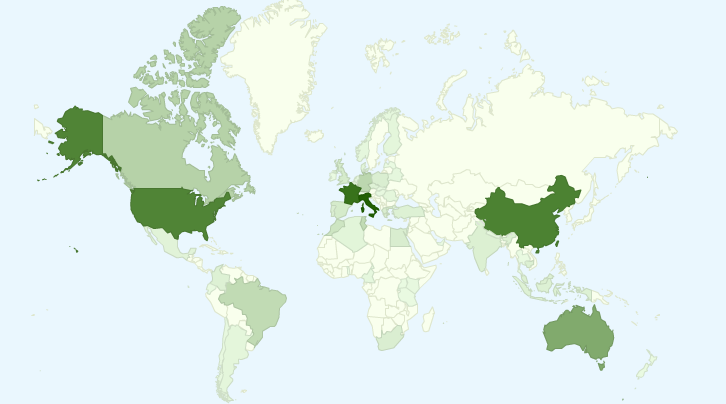
\includegraphics[width=0.9\textwidth]{images/OTB4_download_sourceforge_country_crop.png}\\
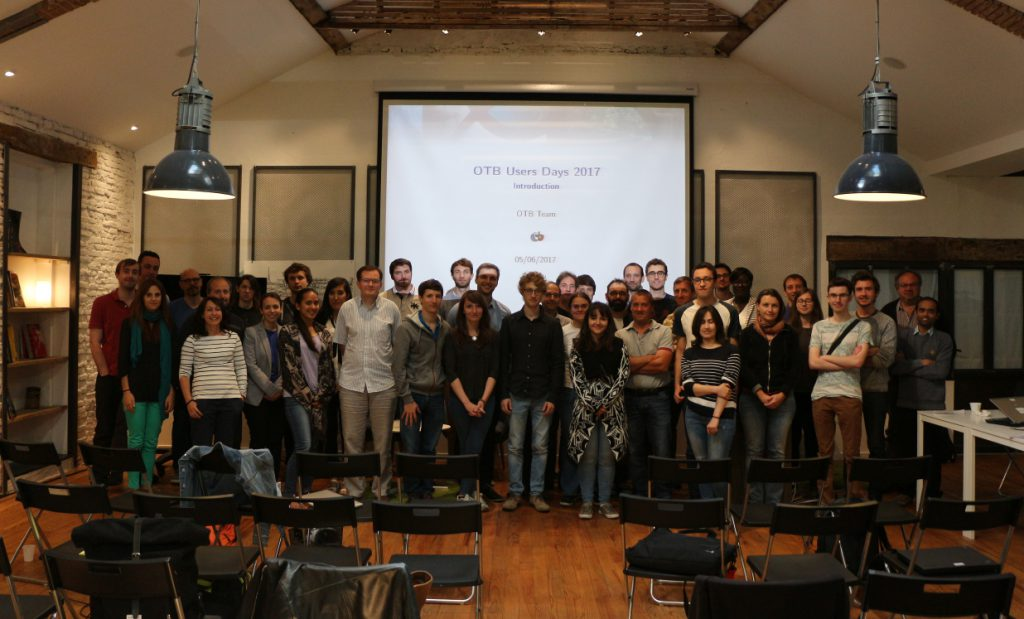
\includegraphics[width=0.9\textwidth]{images/userdays2017.jpg}
\end{columns}

\end{frame}

\begin{frame}
\frametitle{Les réussites de l'OTB}
\vspace{-0.5cm}
\begin{columns}
\column{0.65\textwidth}
\begin{itemize}
\item l'OTB a été utile aux utilisateurs ORFEO et a traité plus de 619 images Pléiades pour le site web RTU,
\item De nombreuses sessions de formation (3 à 5 jours) en France, Belgique, Madagascar, UNESCO, Hawaii, Finlande\ldots
\item L'OTB fournit beaucoup de fonctions utiles pour la télédétection dans un \textbf{unique outil}
\item L'OTB a permis un progrès important du codec JPEG2000 libre OpenJpeg
\item L'OTB égale ou dépasse les outils de l'état de l'art (libre et commercial) pour certaines fonctions:
\begin{itemize}
\item La calculatrice de bandes,
\item La segmentation de scène complètes,
\item La classification à l'échelle d'une scène complète avec un grand choix d'algorithmes,
\item Les ponts entre la télédétection et le systèmes d'information géographique\ldots
\end{itemize}
\item L'OTB est un logiciel officiel OSGeo
\end{itemize}
\column{0.35\textwidth}
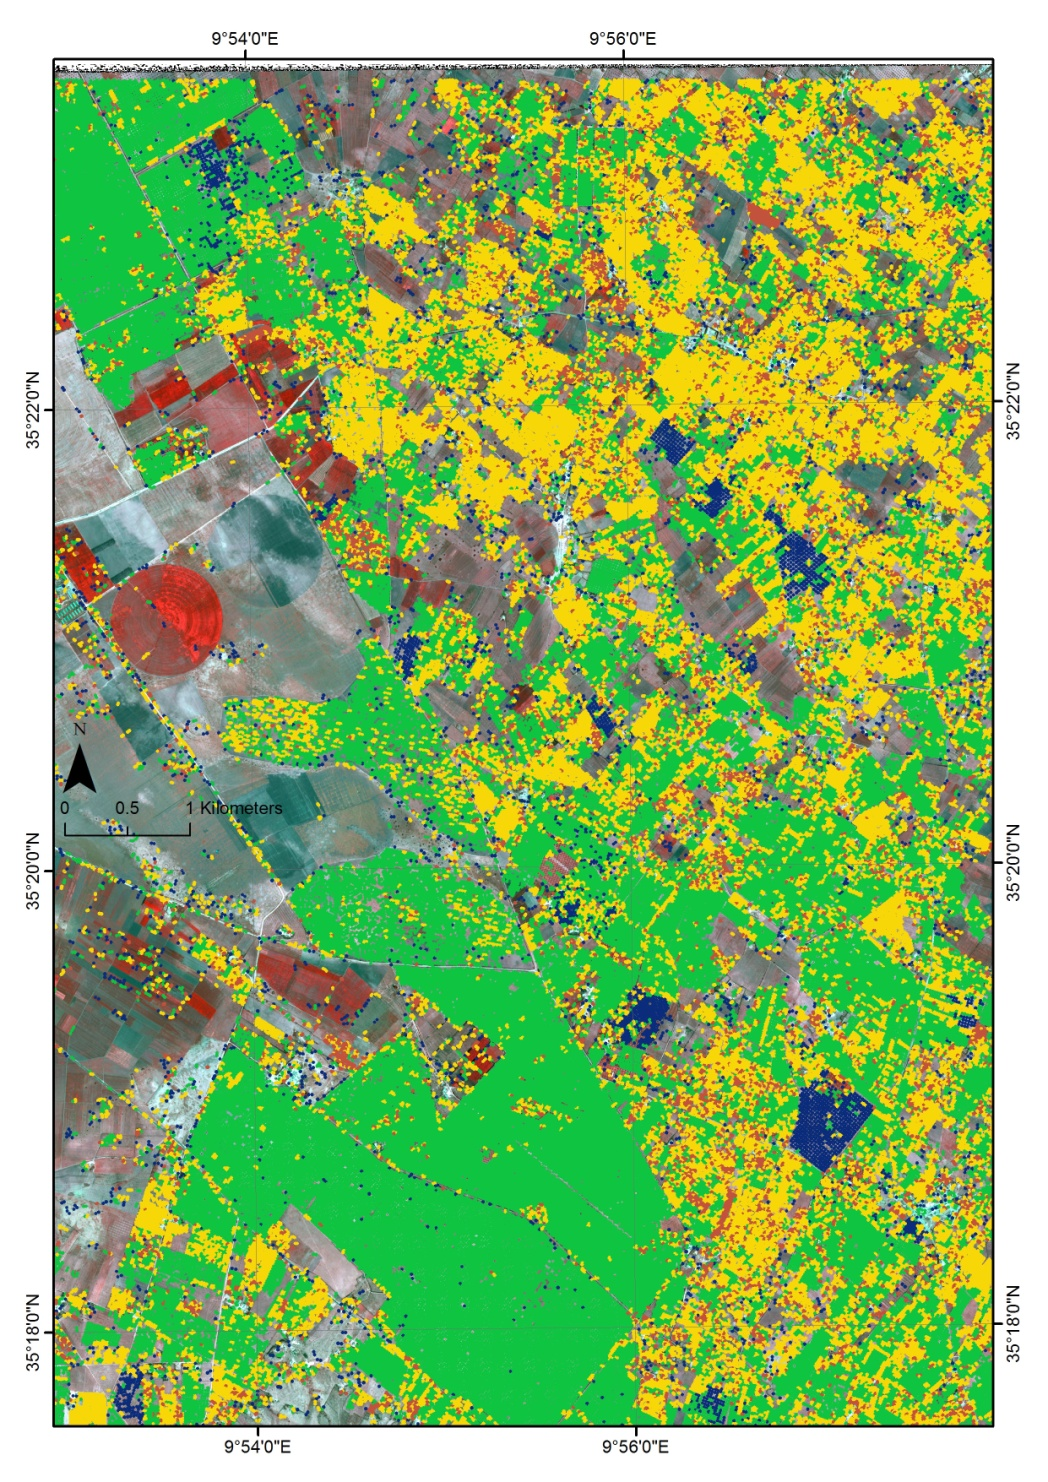
\includegraphics[width=0.9\textwidth]{images/resultats_ird.png}\\
\tiny{Carte thématique à partir d'une segmentation par l'OTB, B. Mougenot~-~IRD}
\end{columns}
\end{frame}

\begin{frame}
  \frametitle{Projets et logiciels utilisant l'OTB}
  \vspace{-0.5cm}
\begin{columns}
  \column{0.55\textwidth}
  \begin{itemize}
    \item Les applications OTB applications sont disponibles dans QGIS et dans Zoo-Project (service WPS)
    \item Certains composant des segments sols S2 et
      Venus (CNES et ESA)
    \item Logiciel éducatif Terr'Image
    \item Produits l'échelle nationale en France
      dans THEIA (Occupation du sol, masques de neige, et même produits 2A via MAJA!)
    \item Projet ESA S2 for Agriculture
    \item Logiciel Gnorasi (National Technical University of Athens)
    \item Projet GEOSUD (IRSTEA)
    \item Programme de recherche TCM (ETS Quebec)
    \item Chaînes de traitement au CEREMA et au SERTIT
  \end{itemize}
  \column{0.6\textwidth}
\begin{center}
  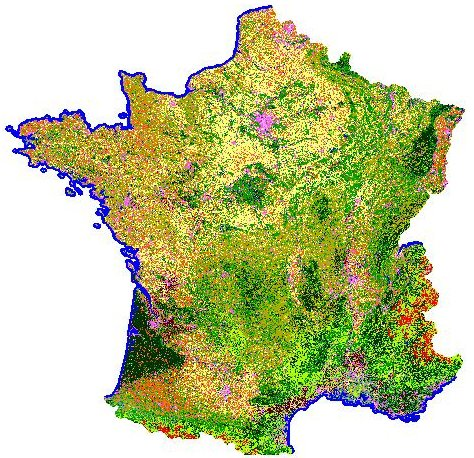
\includegraphics[width=0.6\textwidth,height=0.35\textheight]{images/oso-2017.jpeg}\\
  \tiny{Produit occupation du sol THEIA (CESBIO)}
  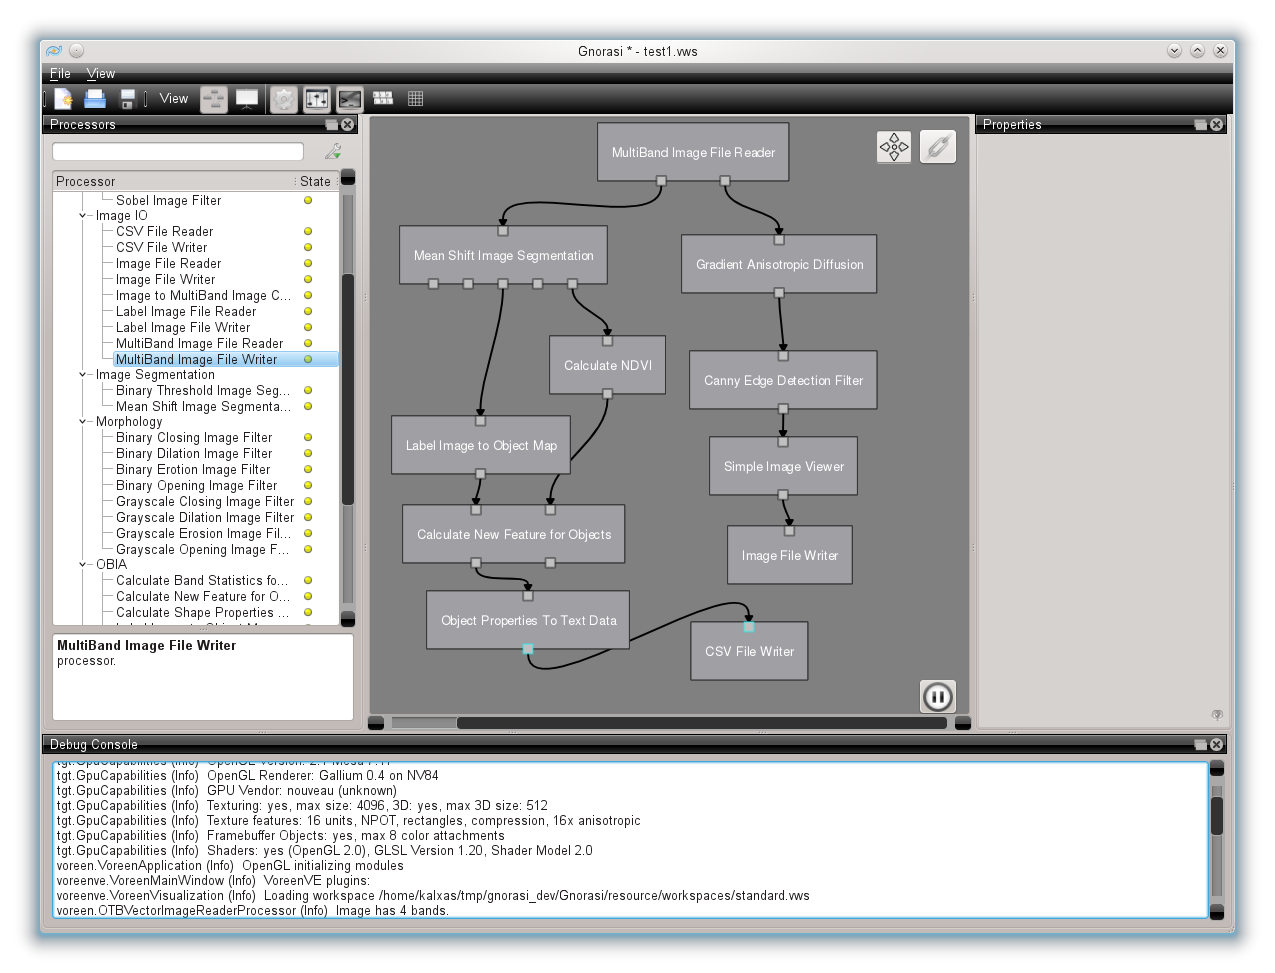
\includegraphics[width=0.6\textwidth]{images/gnorasi2.png}\\
  \tiny{Le logiciel Gnorasi}
\end{center}
\end{columns}
\end{frame}

\begin{frame}
\frametitle{Support/Aide/Contribution}
\vspace{-0.2cm}
\begin{block}{Ressources}
\vspace{-0.2cm}
\begin{description}
\item[Site web] \href{http://www.orfeo-toolbox.org}{orfeo-toolbox.org}
\item[Wiki] \href{http://wiki.orfeo-toolbox.org}{wiki.orfeo-toolbox.org}
\item[Blog] \href{http://blog.orfeo-toolbox.org}{blog.orfeo-toolbox.org}
\end{description}
\end{block}
\vspace{-0.2cm}
\begin{block}{Documentation et aide}
\vspace{-0.2cm}
\begin{description}
\item[Doxygen] \href{http://www.orfeo-toolbox.org/doxygen/}{doxygen}
\item[Documentation] Software Guide et CookBook (remote sensing recipes)
\item[Liste de diffusion utilisateurs] otb-users@googlegroups.com
\item[Liste de diffusion développeurs] otb-developers@googlegroups.com
\end{description}
\end{block}
\vspace{-0.2cm}
\begin{block}{Follow-up}
\vspace{-0.2cm}
\begin{description}
\item[Code, bugs, contributions, feature requests \ldots] \href{https://gitlab.orfeo-toolbox.org/orfeotoolbox/otb}{gitlab.orfeo-toolbox.org}
\item[Météo?] \href{http://dash.orfeo-toolbox.org}{dash.orfeo-toolbox.org}
\end{description}
\end{block}
\end{frame}

\begin{frame}
\frametitle{Merci pour votre attention. Des questions?}
\begin{minipage}[t][6cm][t]{\textwidth}
\begin{center}
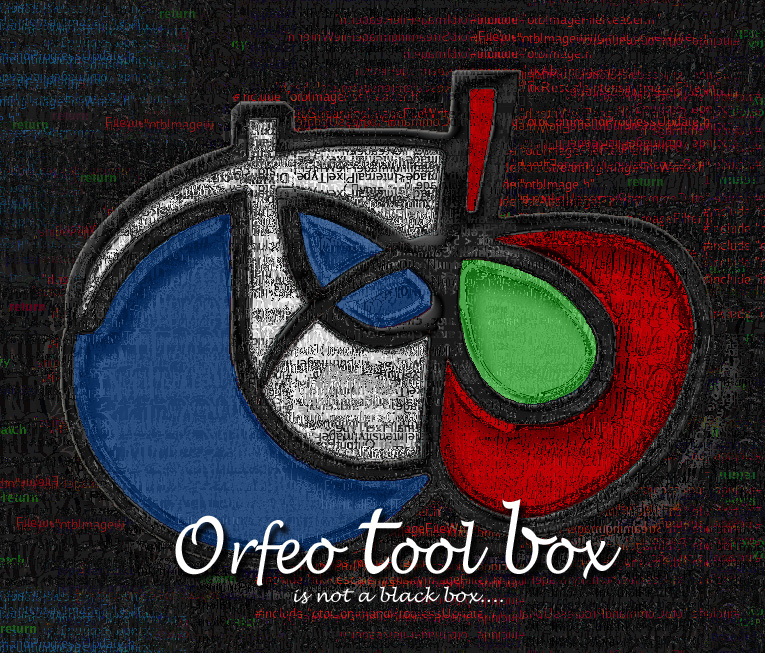
\includegraphics[width=0.65\textwidth]{images/LOGOTB_blackbox.png}
\end{center}
\end{minipage}
\end{frame}
